

\text{ }
\flushleft 30
\center\textbf{КВАНТ} $\cdot$ 2017/№4 

\begin{multicols}{2}
равно $\mathcal{\beta} = x/D$.  Модуль (коэффициент)
объемной упругости G находится из условия

\center3\beta G = \rho_\text{вн}

\flushleft и равен

\center G=-$\frac{\rho_\text{вн}}{3\beta}$=$\frac{24U_0}{D^3}$=$\frac{4L \rho}{M}$=2\rho_\text{соб} .

\center\textbf{Тепловое расширение при
фиксированном внешнем давлении}

\flushleft \hspace{0.3cm}{При колебаниях одной молекулы вблизи среднего положения равновесия в направле-
нии одной из ближайших соседок, в соответ-
ствии с моделью Леннарда–Джонса, должна расти средняя по времени сила отталки-
вания этих двух молекул. Если колебания
описываются (примерно) гармонической
функцией времени $x_{max}cos\omega t$, то для колебаний вдоль оси x изменение потенциальной энергии взаимодействия этой пары молекул
можно описать формулой}

U = U_0((\frac{D}{D+x})^{12}-2(\frac{D}{D+x})^6)\thickapprox 

\center\thickapprox36U_0(\frac{x}{D})^2-252U_0(\frac{x}{D})^3+

\flushright+1113U_0(\frac{x}{D})^4+\ldots .
\flushleft{Сила взаимодействия молекул равна}

\flushleft F(x)=-$\frac{dU}{dx}$\thickapprox-72U_0(\frac{1}{D})^2x+

\center+756U_0(\frac{1}{D})^3x^2-4452U_0(\frac{1}{D})^4x^3+\ldots

\flushleft Среднее значение для $x^2$ при тепловых
колебаниях мы теперь знаем, а третьим
слагаемым, пропорциональным $x^3$, мы пренебрегаем. Чтобы среднее по времени значение силы осталось равным нулю, молекулы
должны в среднем удалиться друг от друга
на расстояние $\Delta \thickapprox 0,146D\textit{k} T/U_0$. Таким образом, при низких температурах тепловой
коэффициент линейного расширения конденсированного вещества равен
\center \gamma = \frac{0.146\kappa}{U_0} .

\flushleft Коэффициент объемного теплового расширения вещества в конденсированном состоянии, естественно, примерно в три раза
больше:
\center 3\gamma = \frac{0.44\kappa}{U_0} \thickapprox \frac{ZR}{5L} .

\columnbreak
\flushleft Если умножить коэффициент объемного
расширения твердого вещества при температуре, составляющей определенную долю
от температуры плавления, например при
$T=T_\text{пл}/10$ , на температуру плавления вещества, то можно получить безразмерные
величины. В таблице 2 приведены относи-

\begin{tabel}
\flushright\caption{\textit{Таблица 2}}   

\begin{tabular}{|p{0,6cm}|p{0,6cm}|p{0,6cm}|p{0,6cm}|p{0,6cm}|p{0,6cm}|p{0,6cm}|p{0,6cm}|p{0,6cm}|}

\hline
   \cellcolor{lightgray}Li & \cellcolor{lightgray}Sn & \cellcolor{lightgray}Be & \cellcolor{lightgray}K & \cellcolor{lightgray}Na & 
   \cellcolor{lightgray}Mg & \cellcolor{lightgray}Pb & \cellcolor{lightgray}Ba & \cellcolor{lightgray}Ti\\
\hline 
    0,60&0,61&0,73 & 0,81 & 0,81 & 0.86 & 0,87 & 0,88 & 0,88\\
\hline
    \cellcolor{lightgray}Mo & \cellcolor{lightgray}W & \cellcolor{lightgray}Tl & \cellcolor{lightgray}Ir & \cellcolor{lightgray}Au & 
    \cellcolor{lightgray}B & \cellcolor{lightgray}Zr & \cellcolor{lightgray}Pt & \cellcolor{lightgray}Ca\\
\hline
0,90&0,95&0,97&1,01&1,03&1,03&1,03&1,04&1,10\\
\hline
    \cellcolor{lightgray}Al & \cellcolor{lightgray}Cd & \cellcolor{lightgray}Cu & \cellcolor{lightgray}Fe & \cellcolor{lightgray}Ag & 
    \cellcolor{lightgray}Ni & \cellcolor{lightgray}Ta & \cellcolor{lightgray}& \cellcolor{lightgray}\\
\hline
    1,11&1,14&1,19&1,19&1,22&1,25&1,25&&\\
\hline
\end{tabular}
\end{tabel}
\flushleft тельные величины $T_\text{пл}\cdot \gamma$ для большой группы металлов. Из таблицы видно, что относительные величины мало отличаются друг
от друга, хотя по механическим и тепловым свойствам (структуре кристаллической
решетки, модулю Юнга, температуре плавления и др.) эти металлы отличаются весьма значительно. Конечно, есть и такие вещества, для которых обсуждаемая относительная величина далеко выходит за границы диапазона 0,6–1,2. Например, она больше для урана (1,8), плутония (2,4), цинка
(2,5), а для галлия (0,31), индия (0,47) и
сурьмы (0,54) она меньше, но эти данные в
таблицу не включены.

\hspace{0.3cm}Следовало бы рассмотреть зависимость
коэффициента объемного расширения от
температуры ( $\gamma$ растет с ростом температуры), но для ее объяснения выбранной модели взаимодействия молекул недостаточно.
\center \textbf{Давление насыщенного пара}
\flushleft
\hspace{0.3cm}Нарисуем зависимости давления одного
моля вещества от занимаемого им объема для
двух немного отличающихся температур T
и $T-\Delta T$ (рис.2). Участки с постоянными
давлениями соответствуют одновременному
существованию в объеме сосуда и конденсированного и газообразного состояния вещества. Кривые пунктирные линии показывают, как вело бы себя это вещество, если бы
оно подчинялось законам идеального газа.

\hspace{0.3cm}Проведем с этим веществом циклический
процесс, в котором две изотермы будут соот-
\end{multicols}
\newpage
\begin{figure}
    \centering
    
\includegraphics[width=1.2\linewidth]{2.png}
    
    \label{fig:enter-label}
\end{figure}
\begin{multicols}{2}
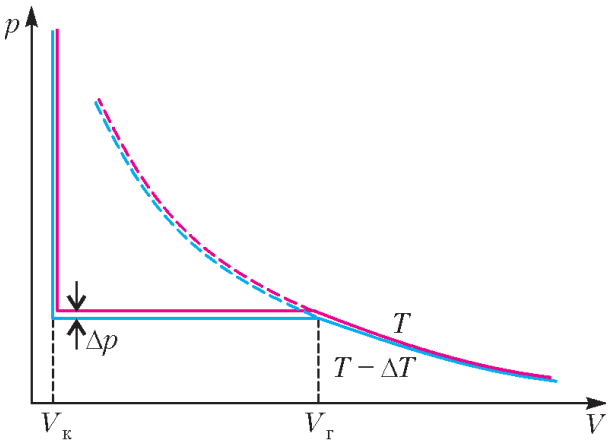
\includegraphics[width=0.90\linewidth]{1.png}
    \flushleft\caption{\textit{Рис. 2}}
    \label{fig:enter-label}

\flushleft  ветствовать испарению вещества при более
высокой температуре и конденсации вещества при более низкой температуре. Соединим эти два участка (на концах) адиабатами.
Получится цикл Карно, для которого КПД
известен – он равен $\Delta T/T$. Теплота, полученная от «нагревателя», соответствует моляр-
\columnbreak
\flushleft Это уравнение (уравнение Клапейрона–Клаузиуса) имеет такое решение:
\center $ln\frac{\rho}{\rho_0}=(\frac{1}{T_0}-\frac{1}{T})\frac{ZL}{Z_0R}+(\frac{i}{2}-1)ln\frac{T_0}{T}$ ,
\flushleft где $\rho_0$
 – давление насыщенного пара вещества при температуре $T_0$.
 
\hspace{0.3cm} Если возвести число $\textit{e}$ в степени, соответствующие правой и левой частям полученного равенства, и оставить по разные стороны
от знака равенства только величины, имеющие одинаковые индексы, то получится соотношение для давления насыщенного пара:
\center
$\rho_\text{нп}T^{\frac{i}{2}-1}\cdotexp(\frac{ZL}{TZ_0R})= const =\Upsilon$ .

\flushleft\hspace{0.3cm} По-видимому, для давлений насыщенного
пара над твердым конденсированным веществом и над жидким величины $\Upsilon$ будут разными.

\hspace{0.3cm} На рисунке 3 для разных веществ приве-
дены зависимости относительных величин
 
\end{multicols}
\end{document}